\documentclass[10pt]{beamer}
\usetheme{Malmoe}
\setbeamertemplate{navigation symbols}{}
\colorlet{beamer@blendedblue}{green!40!black}
\setbeamertemplate{navigation symbols}{}
\newcommand*\oldmacro{}%
\let\oldmacro\insertshorttitle%
\renewcommand*\insertshorttitle{%
\oldmacro\hfill%
\insertframenumber\,/\,\inserttotalframenumber}

\usepackage{caption}
\usepackage{hyperref}
\usepackage[makeroom]{cancel}
\usepackage{ amssymb }
\usepackage{appendixnumberbeamer}
%\usepackage{tikz-feynman}
\usepackage{graphicx}
\begin{document}

\title{Photon Overlap Removal for top FCNC}
\subtitle{$t \rightarrow q \gamma$}
\author[Barkeloo]{Jason Barkeloo}

\titlegraphic{
\includegraphics[width=4cm]{../ATLAS-Logo-Ref-RGB.png}\hspace*{2.75cm}~%
   
\includegraphics[width=4cm]{../uo_logo_green_on_white_2.jpg}
}

\date{April 26, 2018}
\frame{\titlepage}
\frame{\frametitle{Table of Contents}\tableofcontents[hidesubsections]}
\section{Brief Background Top FCNC}


\frame{\frametitle{Top Quark Decays}
\begin{columns}
\begin{column}{0.5\textwidth}
\begin{itemize}
\item Standard model top branching ratio to bW $\simeq 100\%$
\end{itemize}
\centering
 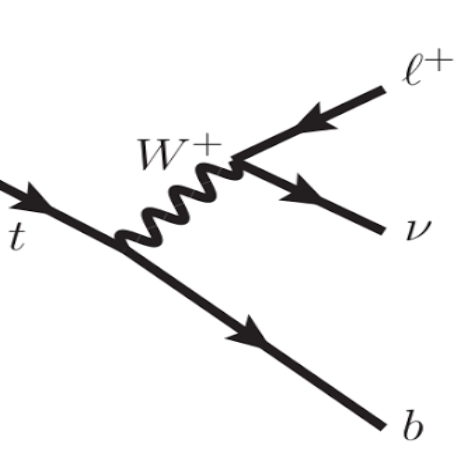
\includegraphics[width=0.7\textwidth]{../../ThesisImages/topdecay.png}
 \captionof{figure}{Leptonic final state diagram for a top decay}
\end{column}
\begin{column}{0.5\textwidth}  %%<--- here
     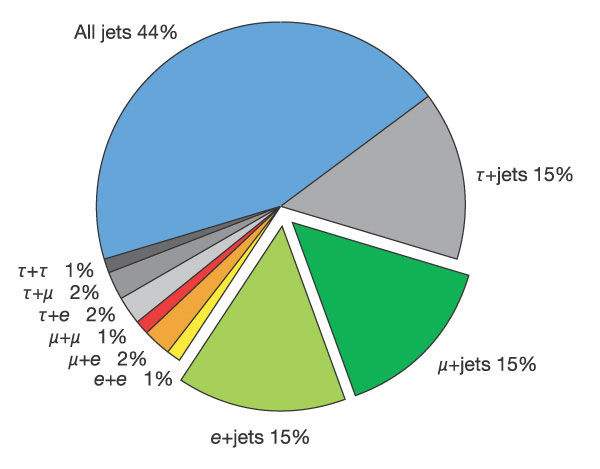
\includegraphics[width=1.1\textwidth]{../../ThesisImages/topdecayproducts.jpg}
    \captionof{figure}{Top quark pair decay final states \href{https://images.nature.com/full/nature-assets/nature/journal/v429/n6992/images/nature02589-f2.2.jpg}{[Nature]}}
\end{column}
\end{columns}
}

\frame{\frametitle{Top Quark Decays in the SM}
\centering
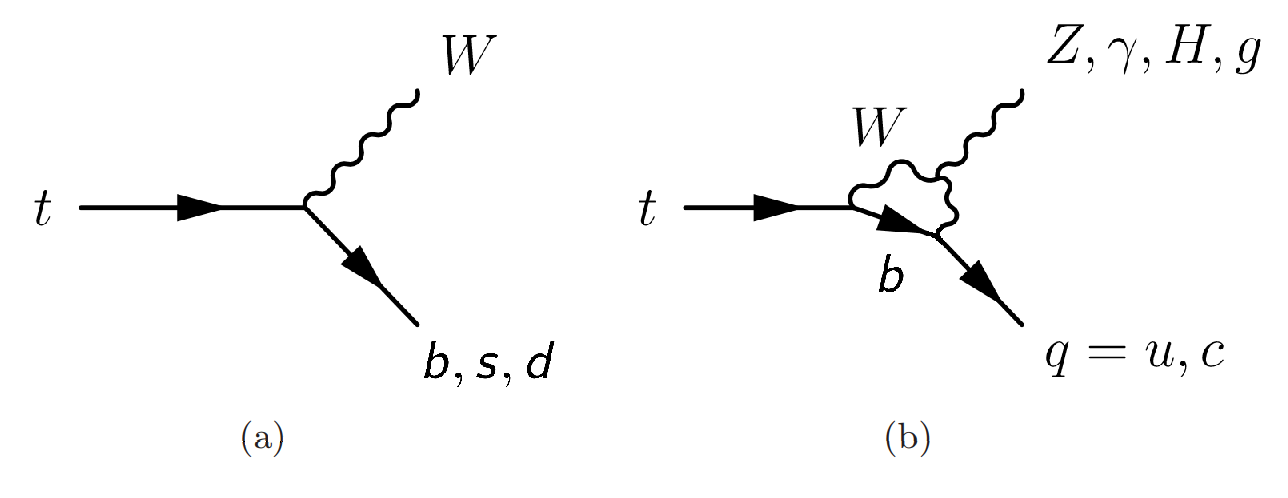
\includegraphics[width=1.\textwidth]{../../ThesisImages/SMTopDecays.png}

\begin{columns}
\begin{column}{0.5\textwidth}
\begin{itemize}
\item $t\rightarrow b W \approx 99.83\%$
\item $t\rightarrow s W \approx 0.16\%$
\item $t\rightarrow d W \approx 0.01\%$
\end{itemize}
\end{column}
\begin{column}{0.5\textwidth}
\begin{itemize}
\item $t\rightarrow q_{u,c} X\approx 10^{-17} - 10^{-12}$
\end{itemize}
\end{column}
\end{columns}


}




\subsection{FCNC at the LHC}
\frame{\frametitle{FCNC: What are we looking for? $t\bar{t}\rightarrow W (\rightarrow l \nu) b+ q\gamma$}
\begin{itemize}
\item Final state topology
	\begin{itemize}
	\item One Neutrino, from W
	\item One Lepton, from W
	\item One B-jet, SM top
	\item \textbf{One Photon, FCNC Top}
	\item One Jet, FCNC Top
	\end{itemize}
\end{itemize}
\centering
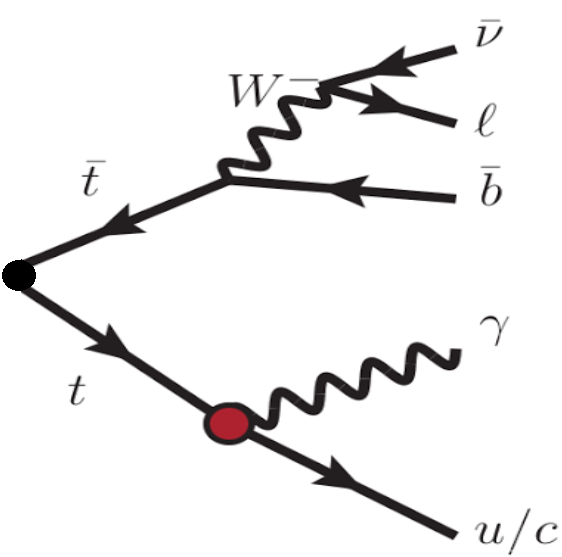
\includegraphics[width=0.4\textwidth]{../../ThesisImages/fcncttbar.png}
}

\frame{\frametitle{Background Processes}
\begin{itemize}
\item Due to all of the processes at hadron colliders it is important to model similar event topologies well.
\item Major backgrounds include $t\bar{t}$, W+Jets, Z+Jets, + processes with an associated photon
\end{itemize}
\centering
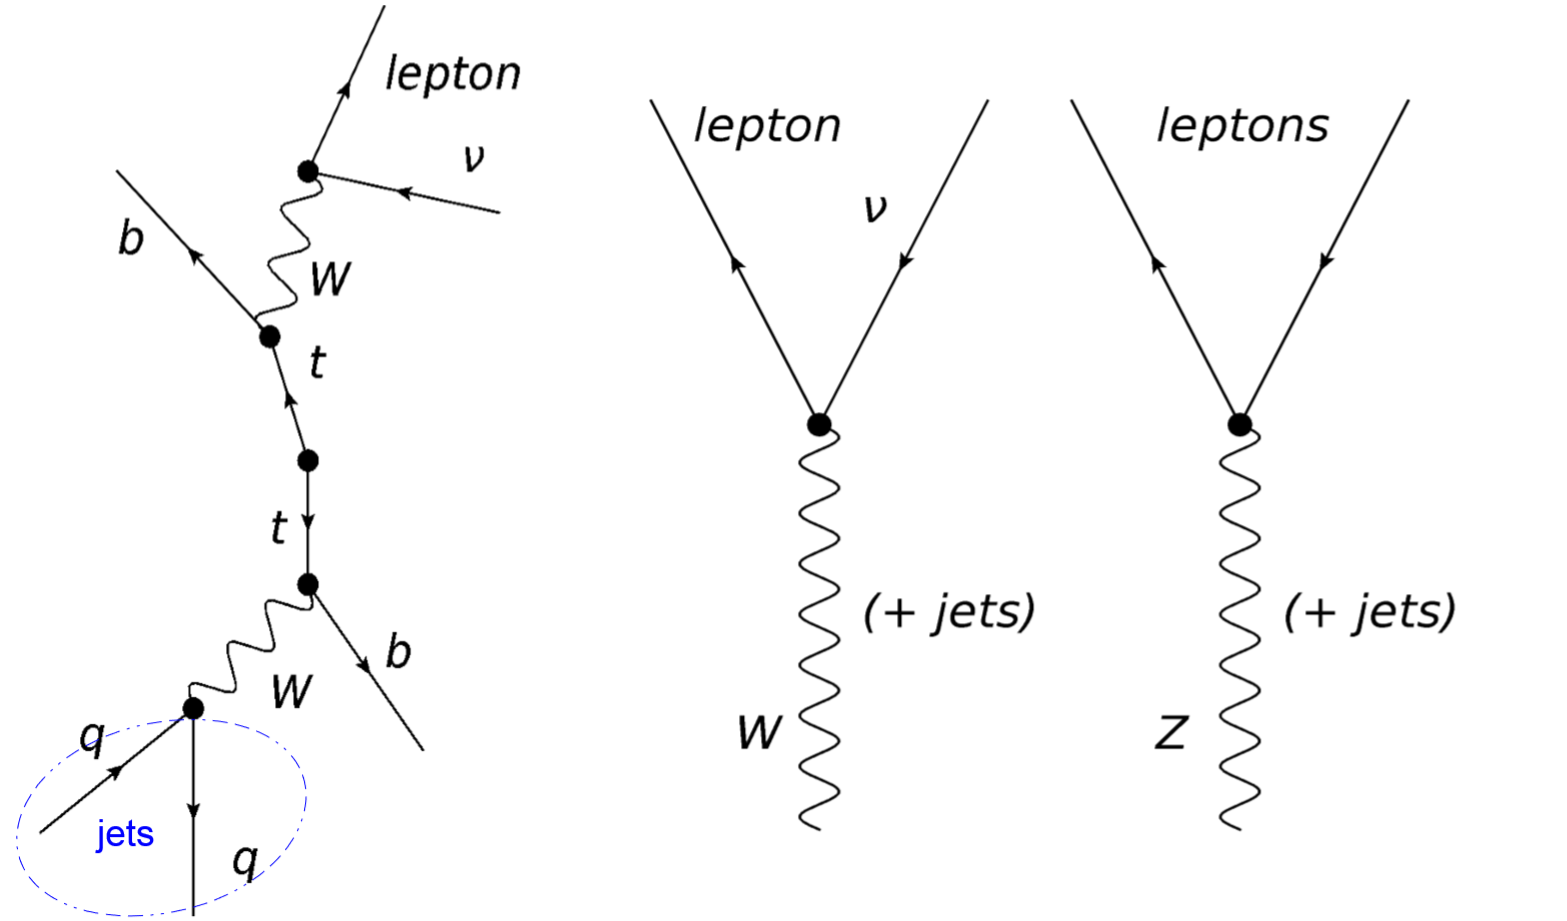
\includegraphics[width=0.7\textwidth]{../../ThesisImages/backgrounds.png}
}

\frame{\frametitle{Monte Carlo Generation}
\begin{itemize}
\item All of our MC data is put through a showering algorithm for propagation from final decay states
\item Various showering algorithms are used at ATLAS - Pythia, Herwigg, etc.
\item All of these will add radiative photons
\item These events can be contained in other samples with explicit photons originating from the hard interaction
\item Need to remove these events or risk double counting events
\end{itemize}

}


%%%%%%%%%%%%%%%%%%%%%%%%%%%%%%%%%%%%%%%%%%%%%%%%%%%%%%%%%%%%%%%%%
\section{Overlap Removal Implementation}

\subsection{Ways of producing photons}
\frame{\frametitle{Photon Overlap Removal}
\begin{itemize}
\item Truth matching procedure is used to identify origin and type of truth particle corresponding to reconstructed photon
	\begin{itemize}
	\item If reco photon is associated with a truth electron or within R=0.2  we can consider this $e\rightarrow \gamma$ fake
	\item If origination from boson or lepton with a corresponding truth hadron: hadron fake
	\item Otherwise the photon is considered coming from the hard interaction
	\item The procedure rejects less than 1\% of events in $t\bar{t}+\gamma$ and $V+\gamma$ samples (except $Z+\gamma$ in e+jets channel because of fake rates)
	\end{itemize}
\end{itemize}
}


\frame{\frametitle{Photon Overlap Removal}
\begin{itemize}

\item For $t\bar{t}$ and $V+jets$ samples, the prompt photon contribution is subject to large statistical uncertainty and its modelling is less trusted, it is why the $t\bar{t}+\gamma$ and $V+\gamma$ samples are used. 
\item For this to work phase spaces of events must be close to identical otherwise the overlap removal will take out too much
\end{itemize}
\centering
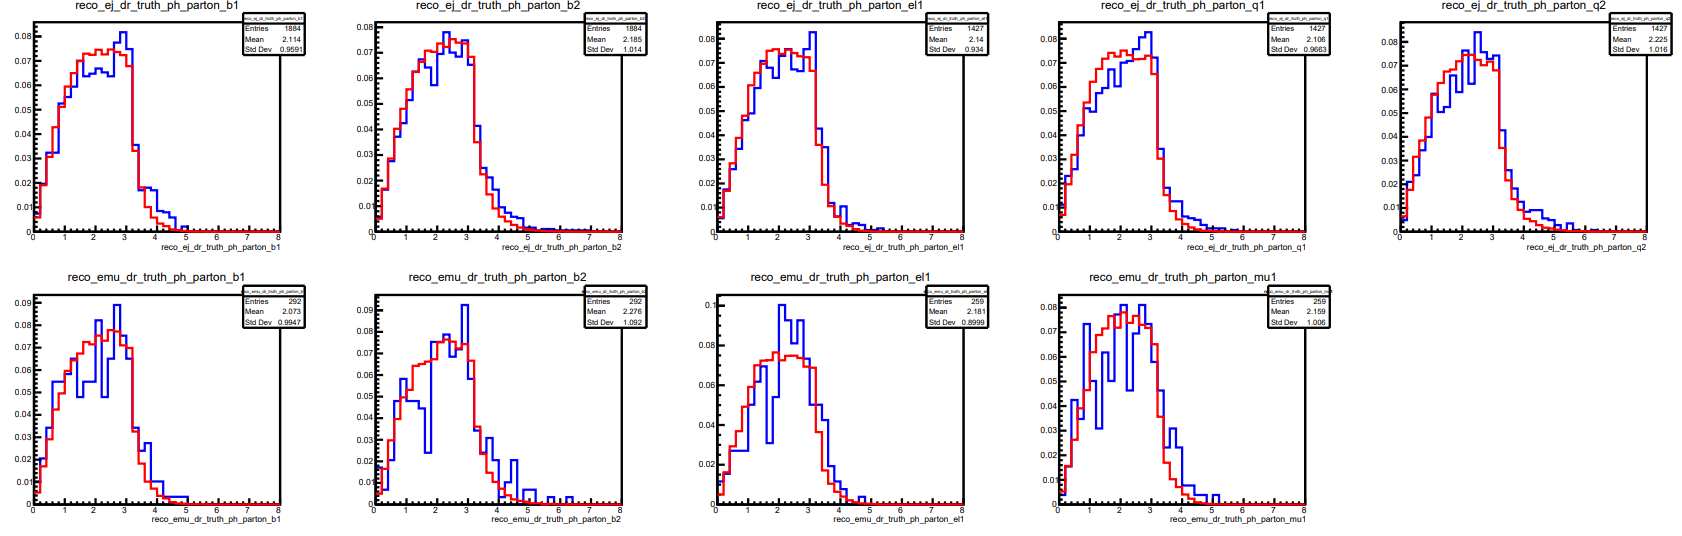
\includegraphics[width=0.9\textwidth]{../../ThesisImages/OverlapRemovalTTgam.png}
\captionof{figure}{Overlaping Phase Space Regions of the photon and various objects \href{https://indico.cern.ch/event/702559/contributions/2882085/attachments/1593846/2523500/main2.pdf}{[Y.Li]} Red: $t\bar{t}+\gamma$ Blue: $t\bar{t}$}
}

\subsection{FCNCs with Photons}

\subsection{Object Preselection Cuts}


\frame{\frametitle{Object Preselection}
\begin{itemize}
\item We preselect events with objects that look like our expected topology
\item Reminder that I require:
	\begin{itemize}
	\item Exactly one lepton (e or $\mu$) $\geq$ 28 GeV
	\item Exactly one Good photon $\geq$ 25GeV
	\item Missing Transverse Energy $\geq$ 30GeV
	\item $\geq 2$ Jets (at least one being b-tagged)
	\end{itemize}
\item All following plots will have signal scaled to $0.2\%$ of nonallhadronic $\sigma_{t\bar{t}}$, MC scaled to $36.07fb^{-1}$
\item Only electron channel shown.  Similar results for the muon channel are seen.
\end{itemize}
}


\frame{\frametitle{Preselection Objects}

\begin{columns}
\begin{column}{0.02\textwidth}

\rotatebox{90}{W/OVR \qquad  \qquad No OVR} 
%\rotatebox{90}{Muon Channel        } 
\end{column}
\begin{column}{0.33\textwidth}
\begin{itemize}
\item  Leading Jet $p_T$
\end{itemize}
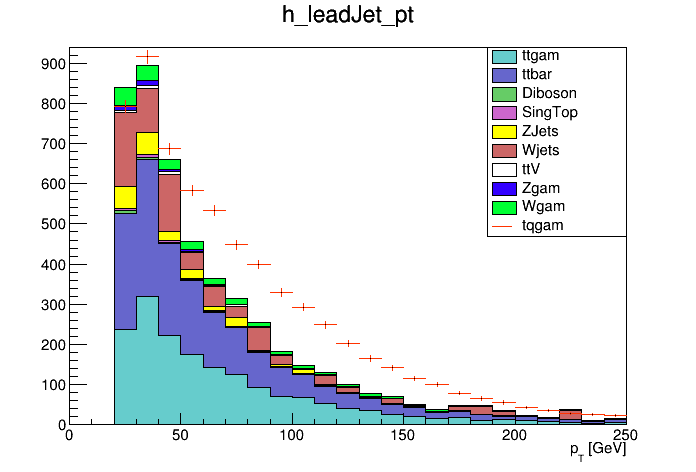
\includegraphics[width=1.1\textwidth]{../../ThesisImages/plotsloose/el_h_leadJet_pt.png} \\
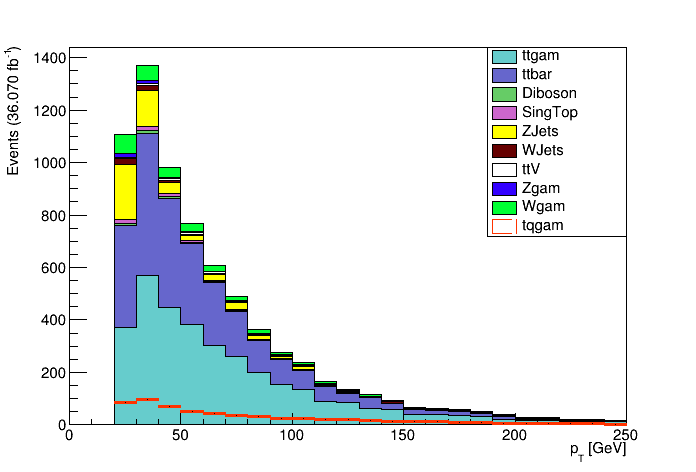
\includegraphics[width=1.1\textwidth]{../../ThesisImages/OverlapRemovalNoRegion/plots/el_presel/el_preselh_leadJet_pt.png}
\end{column}
\begin{column}{0.33\textwidth}
\begin{itemize}
\item Photons
\end{itemize}
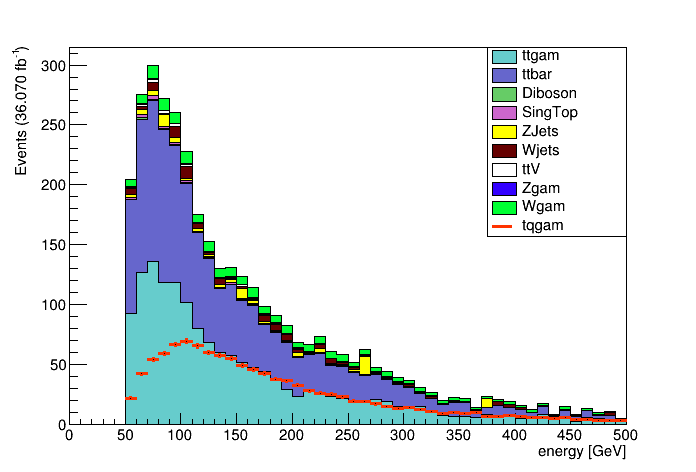
\includegraphics[width=1.1\textwidth]{../../ThesisImages/plotsloose/el_h_photon_e.png} \\
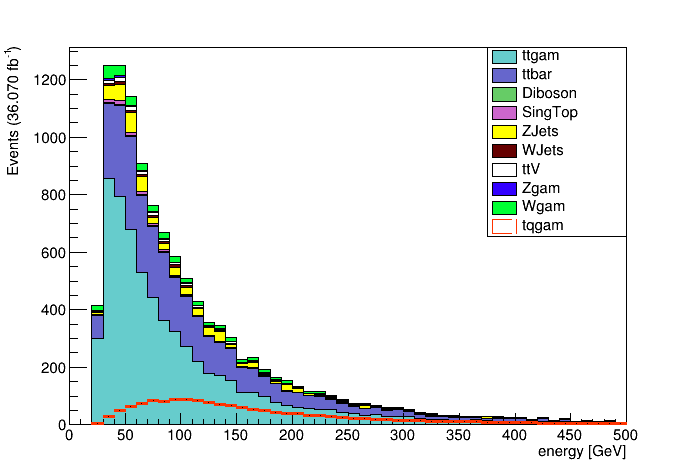
\includegraphics[width=1.1\textwidth]{../../ThesisImages/OverlapRemovalNoRegion/plots/el_presel/el_preselh_photon_e.png}
\end{column}
\begin{column}{0.33\textwidth}
\begin{itemize}
\item Leptons
\end{itemize}
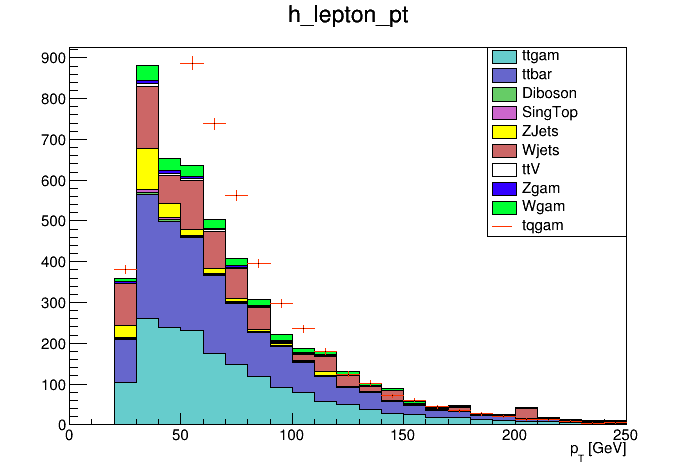
\includegraphics[width=1.1\textwidth]{../../ThesisImages/plotsloose/el_h_lepton_pt.png}\\
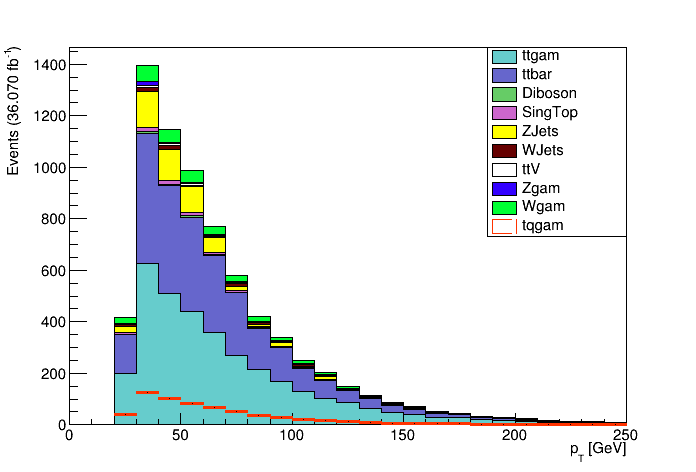
\includegraphics[width=1.1\textwidth]{../../ThesisImages/OverlapRemovalNoRegion/plots/el_presel/el_preselh_lepton_pt.png}
\end{column}
\end{columns}
}


\subsection{Overlap Removal Implications}
\frame{\frametitle{What does this mean?}
\begin{itemize}
\item Previous presentations have dramatically overcounted $t\bar{t}$ events
\item $40-50\%$ of the events in $t\bar{t}$ and $W+jets$ base samples are removed with this procedure
\item The inclusion could have hidden some potential differences in ways to remove one or the other background processes
\end{itemize}
\begin{columns}
\begin{column}{0.5\textwidth}
\centering
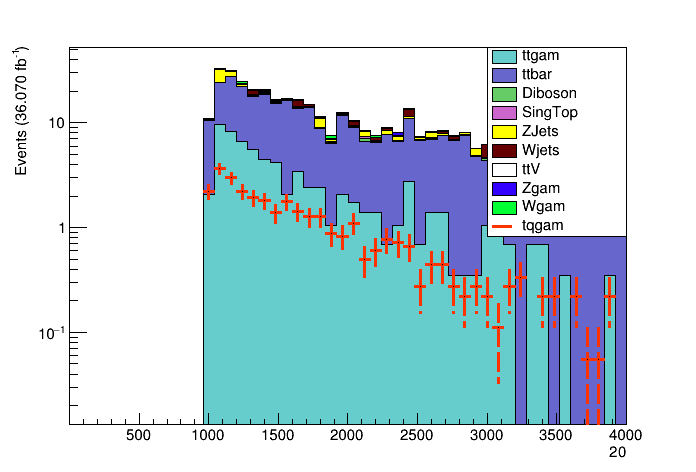
\includegraphics[width=.9\textwidth]{../../ThesisImages/plotsloose/el_h_ph_ptvarcone20.png}
\captionof{figure}{No OVR Photon ptcone20}
\end{column} 
\begin{column}{0.5\textwidth}
\centering
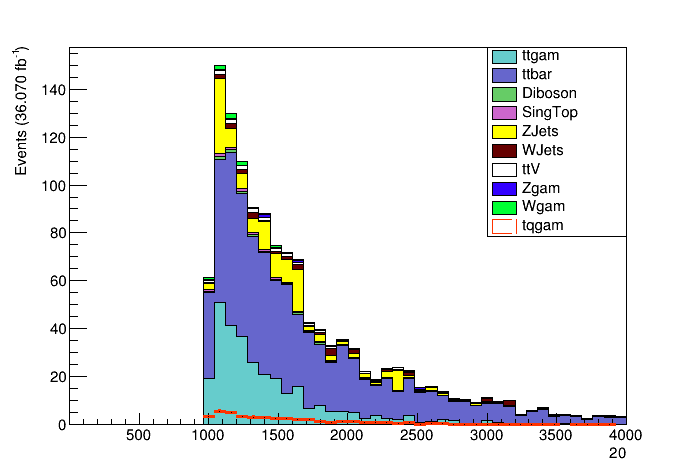
\includegraphics[width=.9\textwidth]{../../ThesisImages/OverlapRemovalNoRegion/plots/el_presel/el_preselh_ph_ptvarcone20.png}
\captionof{figure}{OVR Photon ptcone20}
\end{column}
\end{columns}
}

%%%%%%%%%%%%%%%%

\frame{\frametitle{Other Variables}
\begin{columns}
\begin{column}{0.02\textwidth}
\rotatebox{90}{W/OVR \qquad  \qquad No OVR} 
\end{column}
\begin{column}{0.5\textwidth}
\begin{itemize}
\item  $\Delta R_{\gamma l}$
\end{itemize}
\centering
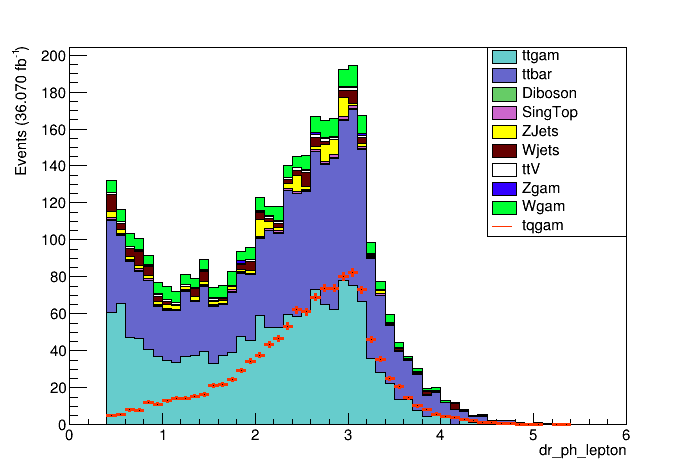
\includegraphics[width=.9\textwidth]{../../ThesisImages/plotsloose/el_h_ph_drlepton.png}\\
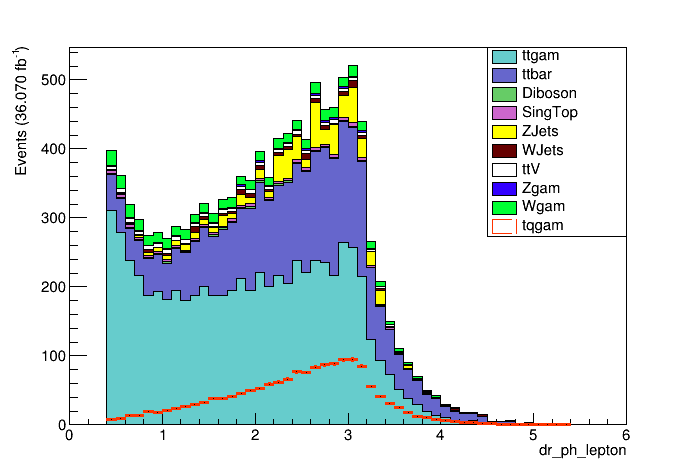
\includegraphics[width=.9\textwidth]{../../ThesisImages/OverlapRemovalNoRegion/plots/el_presel/el_preselh_ph_drlepton.png}
\end{column} 
\begin{column}{0.5\textwidth}
\begin{itemize}
\item $\gamma_\Theta$
\end{itemize}
\centering
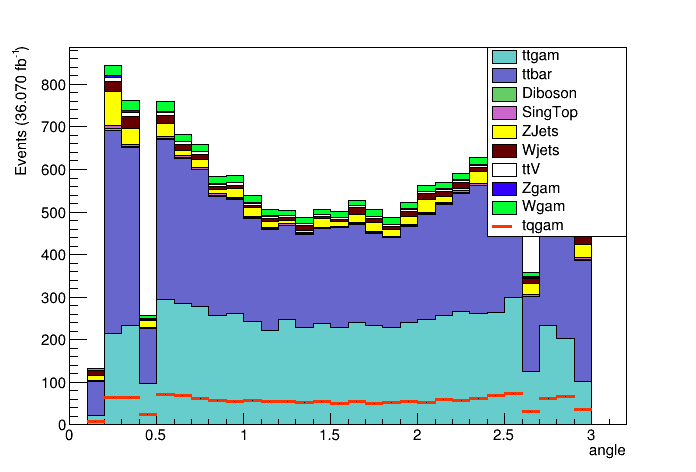
\includegraphics[width=.9\textwidth]{../../ThesisImages/plotsloose/el_h_photon_theta.png}\\
\includegraphics[width=.9\textwidth]{../../ThesisImages/OverlapRemovalNoRegion/plots/el_presel/el_preselh_photon_theta.png}
\end{column}
\end{columns}
}

\section{Current Status, Region Implementation}
\subsection{Region Creation}

\frame{\frametitle{Signal Region}
\begin{itemize}
\item Current Requirements:
	\begin{itemize}
	\item Preselection Cuts
	\item FCNC Top Mass: $m_{q\gamma}$ within 50GeV of $m_t$
	\item SM Top Mass: $m_{b l \nu}$ within 50GeV of $m_t$
	\item Z Mass: $m_{l \gamma} >10GeV$ from $m_Z$
	\item Photon pt $> 50GeV$
	\item ==1 Bjet
	\end{itemize}
\end{itemize}
}

\frame{\frametitle{Some SR Variables}
\begin{columns}
\begin{column}{0.02\textwidth}
\rotatebox{90}{SR Cuts \qquad  \qquad PreSelection} 
\end{column}
\begin{column}{0.5\textwidth}
\begin{itemize}
\item  $\Delta R_{l \gamma}$
\end{itemize}
\centering
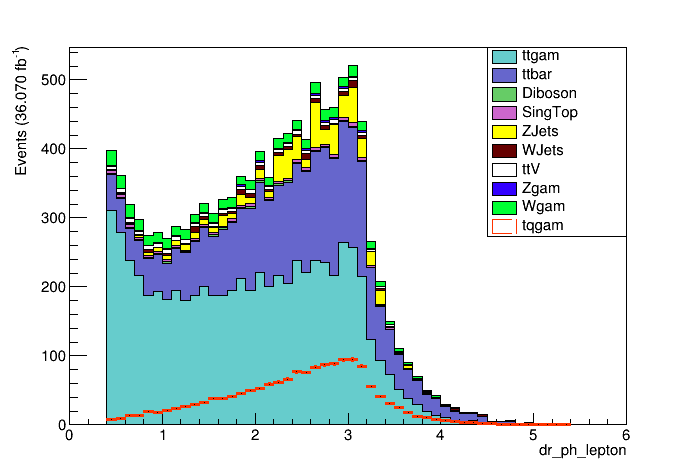
\includegraphics[width=.9\textwidth]{../../ThesisImages/OverlapRemovalNoRegion/plots/el_presel/el_preselh_ph_drlepton.png}\\
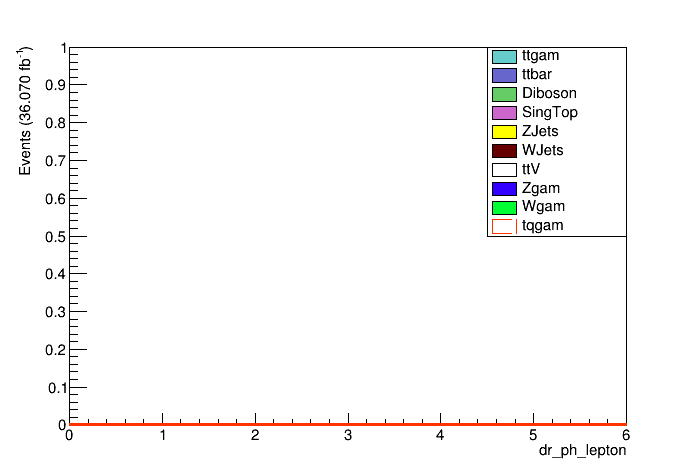
\includegraphics[width=.9\textwidth]{../../ThesisImages/OverlapRemovalRegions/plots/el_SR/el_SRh_ph_drlepton.png}
\end{column} 
\begin{column}{0.5\textwidth}
\begin{itemize}
\item $\gamma_\Theta$
\end{itemize}
\centering
\includegraphics[width=.9\textwidth]{../../ThesisImages/OverlapRemovalRegions/plots/el_presel/el_preselh_photon_theta.png}\\
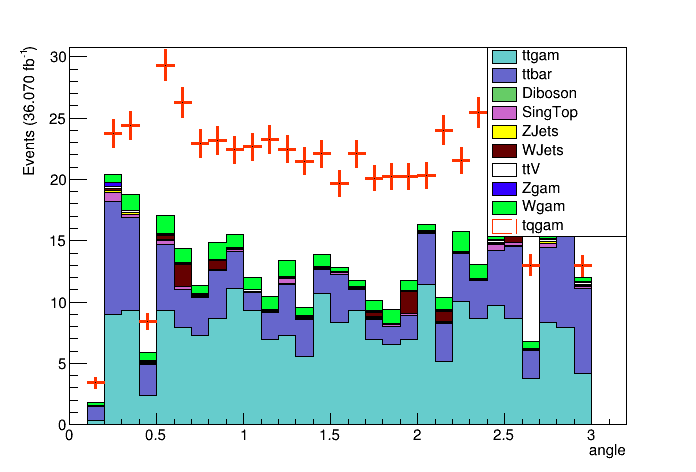
\includegraphics[width=.9\textwidth]{../../ThesisImages/OverlapRemovalRegions/plots/el_SR/el_SRh_photon_theta.png}
\end{column}
\end{columns}
}

\frame{\frametitle{Some More SR Variables}
\begin{columns}
\begin{column}{0.02\textwidth}
\rotatebox{90}{SR Cuts \qquad  \qquad PreSelection} 
\end{column}
\begin{column}{0.5\textwidth}
\begin{itemize}
\item  $m_{q \gamma}$
\end{itemize}
\centering
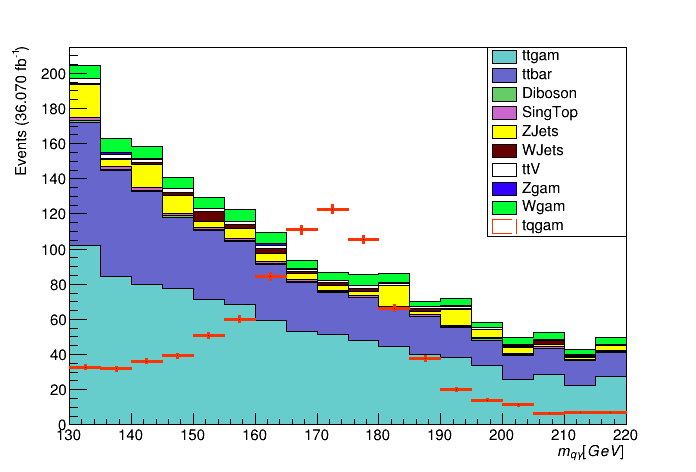
\includegraphics[width=.9\textwidth]{../../ThesisImages/OverlapRemovalNoRegion/plots/el_presel/el_preselh_qgam_m.png}\\
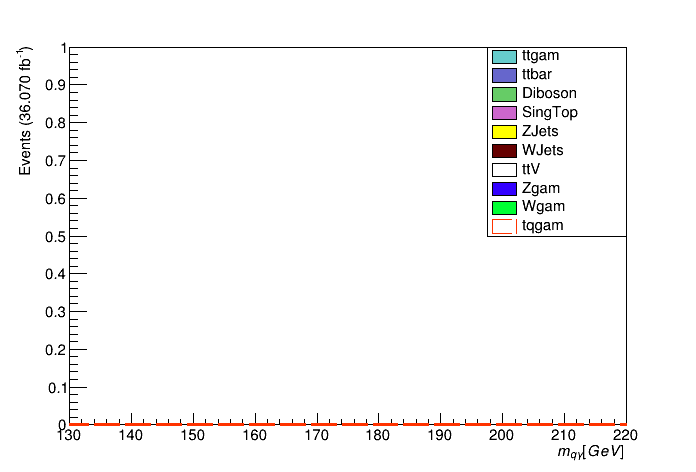
\includegraphics[width=.9\textwidth]{../../ThesisImages/OverlapRemovalRegions/plots/el_SR/el_SRh_qgam_m.png}
\end{column} 
\begin{column}{0.5\textwidth}
\begin{itemize}
\item $m_{bl\nu}$
\end{itemize}
\centering
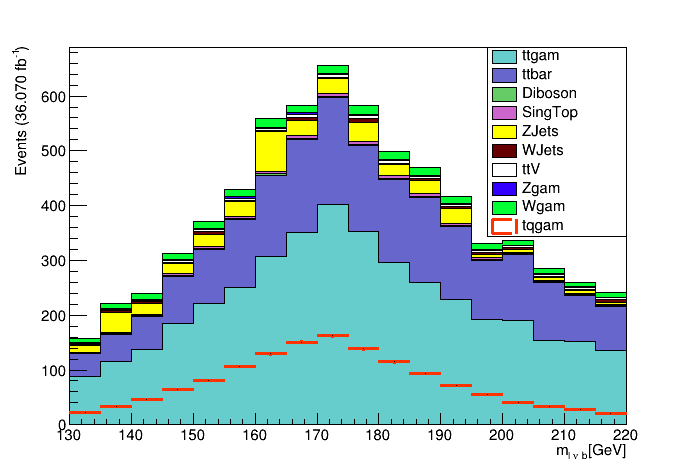
\includegraphics[width=.9\textwidth]{../../ThesisImages/OverlapRemovalNoRegion/plots/el_presel/el_preselh_sm_top_m.png}\\
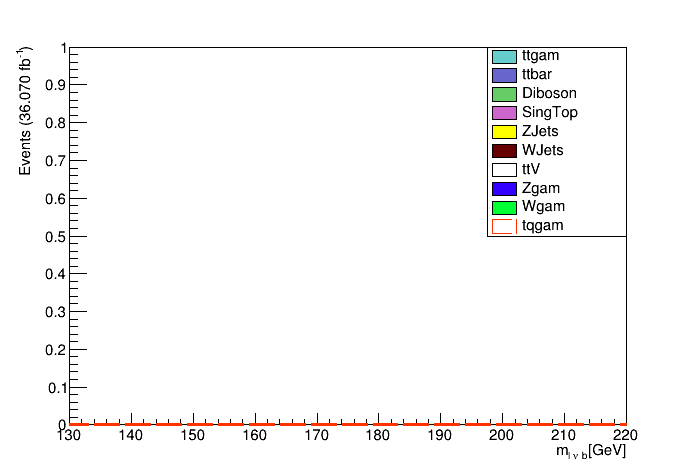
\includegraphics[width=.9\textwidth]{../../ThesisImages/OverlapRemovalRegions/plots/el_SR/el_SRh_sm_top_m.png}
\end{column}
\end{columns}
}

\frame{\frametitle{$t\bar{t}+\gamma$ rich region}
\begin{itemize}
\item Preselection Cuts
\item FCNC Top Mass - Orthogonal to SR
\item $\geq 4$ Jets
\end{itemize}
\begin{columns}
\begin{column}{0.5\textwidth}
\centering
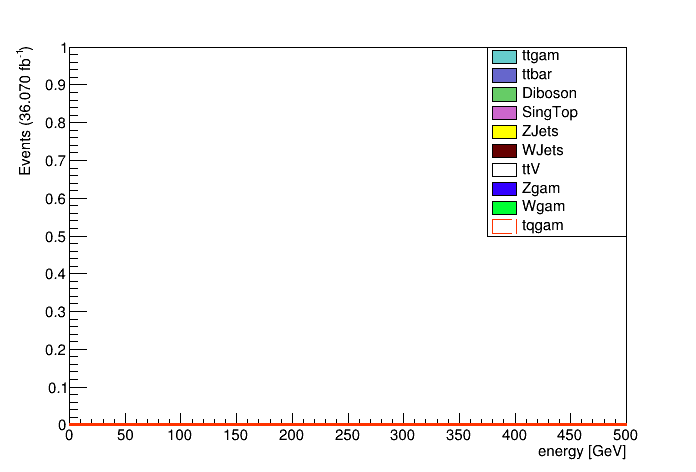
\includegraphics[width=.9\textwidth]{../../ThesisImages/OverlapRemovalRegions/plots/el_VR2/el_VR2h_photon_e.png}
\captionof{figure}{$\gamma_e$}
\end{column} 
\begin{column}{0.5\textwidth}
\centering
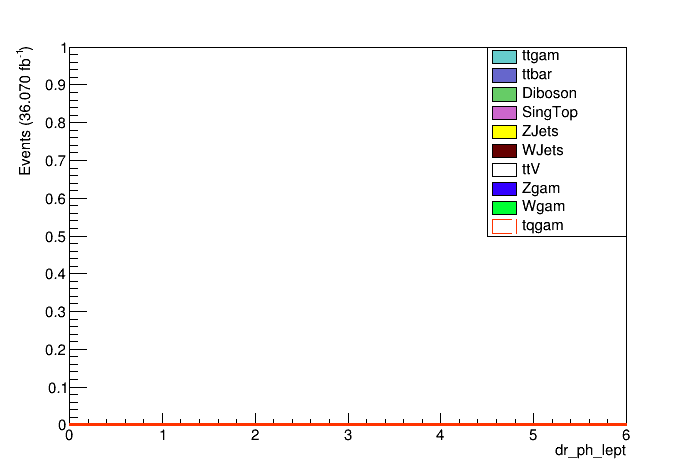
\includegraphics[width=.9\textwidth]{../../ThesisImages/OverlapRemovalRegions/plots/el_VR2/el_VR2h_ph_drlept.png}
\captionof{figure}{$\Delta R_{l \gamma}$}
\end{column}
\end{columns}
}


\frame{\frametitle{Other Regions}
\begin{itemize}
\item Developing more region to test the performance of MC samples
\item Regions are designed to isolate various physics processes using orthogonal selections
\item $t\bar{t}(+\gamma)$ is of utmost important to model extremely well, especially with the increase in cross section at 13TeV
\end{itemize}
}

%%%%

%%%%%%%%%%%%%%%%%%%%%%%%%%%%%%%%%%%%%%%%%%%%%%%%%%%%%%%%%%%%%%%%%%
\section{}

\subsection{Conclusion}
\frame{\frametitle{Conclusion, Outlook}
\begin{itemize}
\item Orthogonal validation/control regions are in development
\item Data grid run complete, need to incorporate into CR/VR plots
\item Next grid run will include a couple of looser regions for CR/VRs 
	\begin{itemize}
	\item 0 Photon Samples for Backgrounds with no Real Photons
	\item 0 BJet Samples - possibly for WJets region
	\end{itemize}
\item Top Group - Pushing for MVA, want to start investigations using these techniques 
\end{itemize}
}


%%%%%%%%%%%%%%%%%%%%%%%%%%%%%%%%%%%%%%%%%%%%%%%%%%%%%%%%%%%%%%%%
%%%%%%%%%%%%%%%%%%%%%%%%%%%%%%%%%%%%%%%%%%%%%%%%%%%%%%%%%%%%%%%% 	
\appendix
\section{Backup}
\frame{\frametitle{Backup}
}
\frame{\frametitle{Integrated Luminosity}
\centering
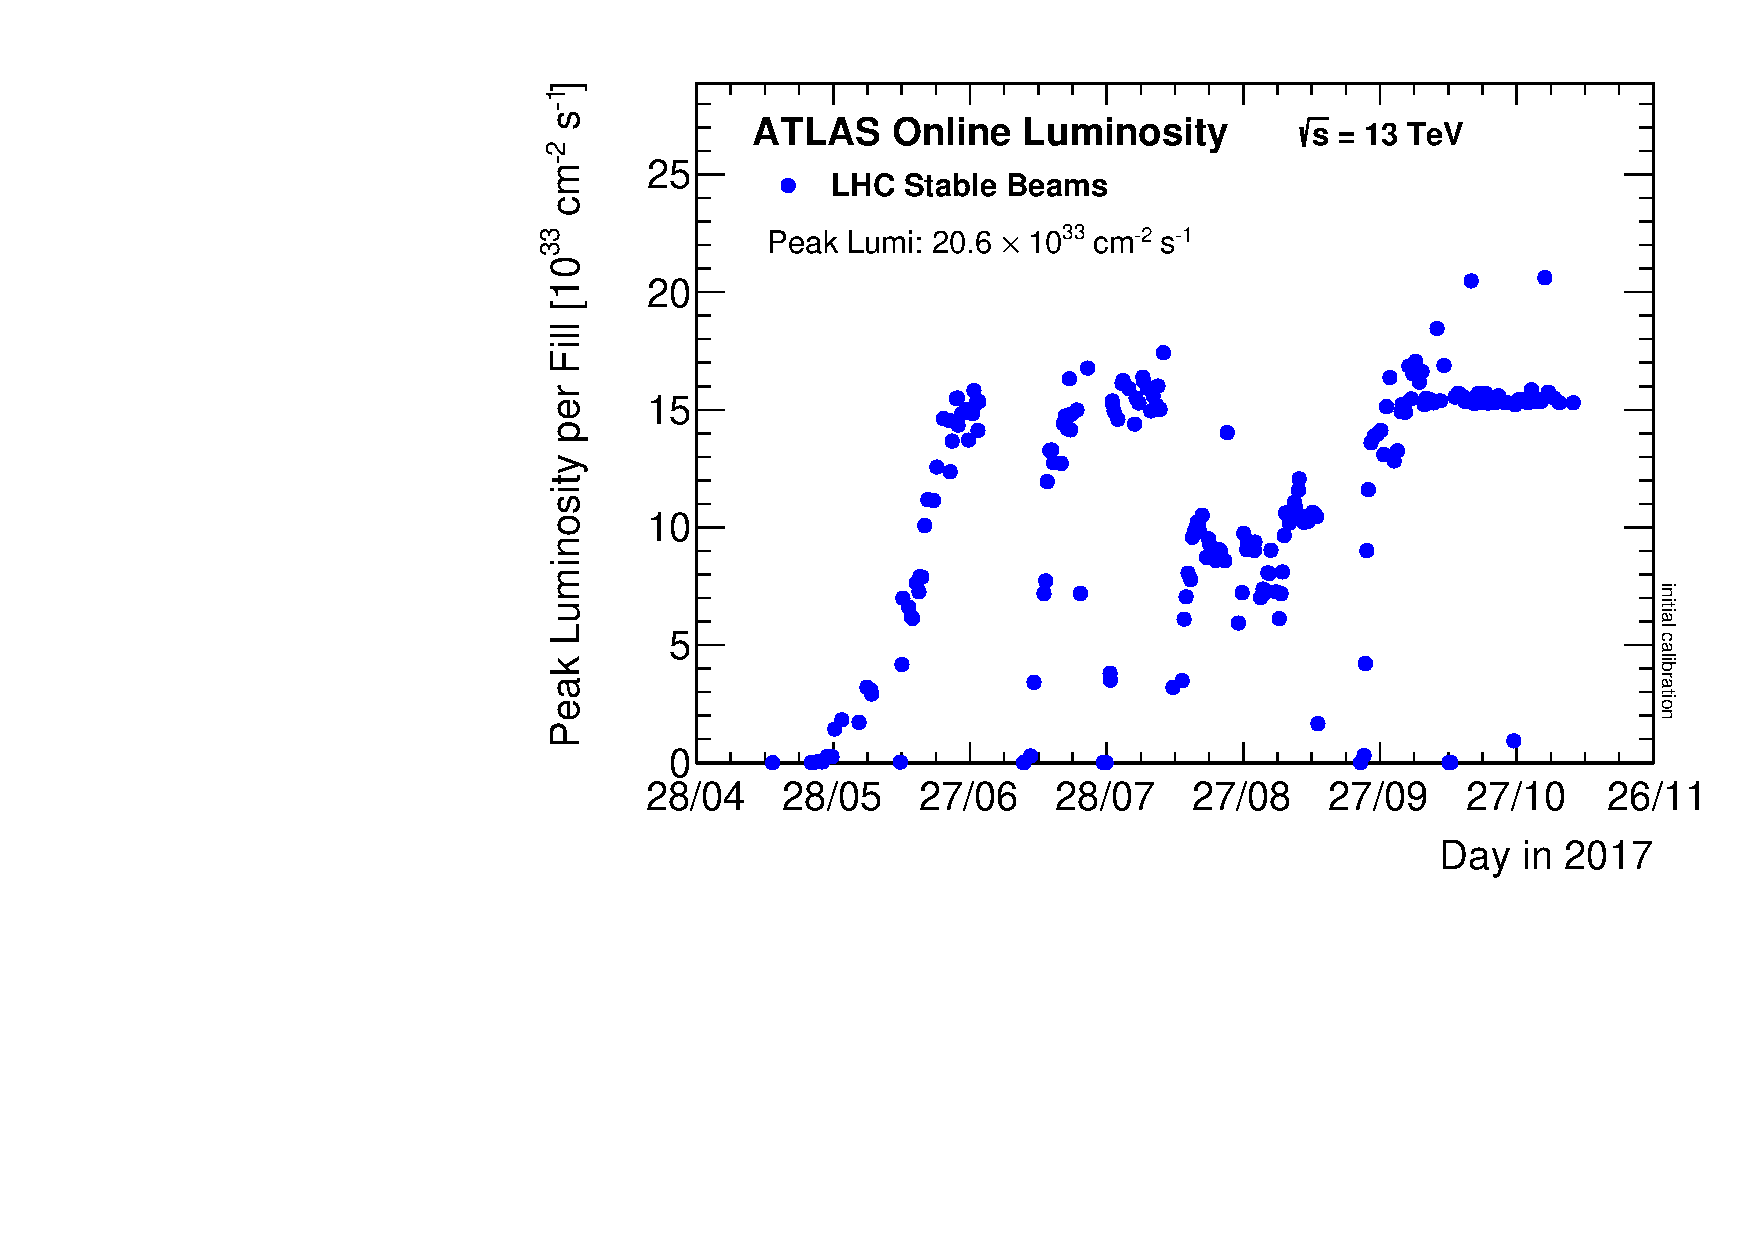
\includegraphics[width=1.\textwidth]{../../ThesisImages/2017PeakLumiByFill.pdf}
}
\frame{\frametitle{A Couple BSM Diagrams}
\centering
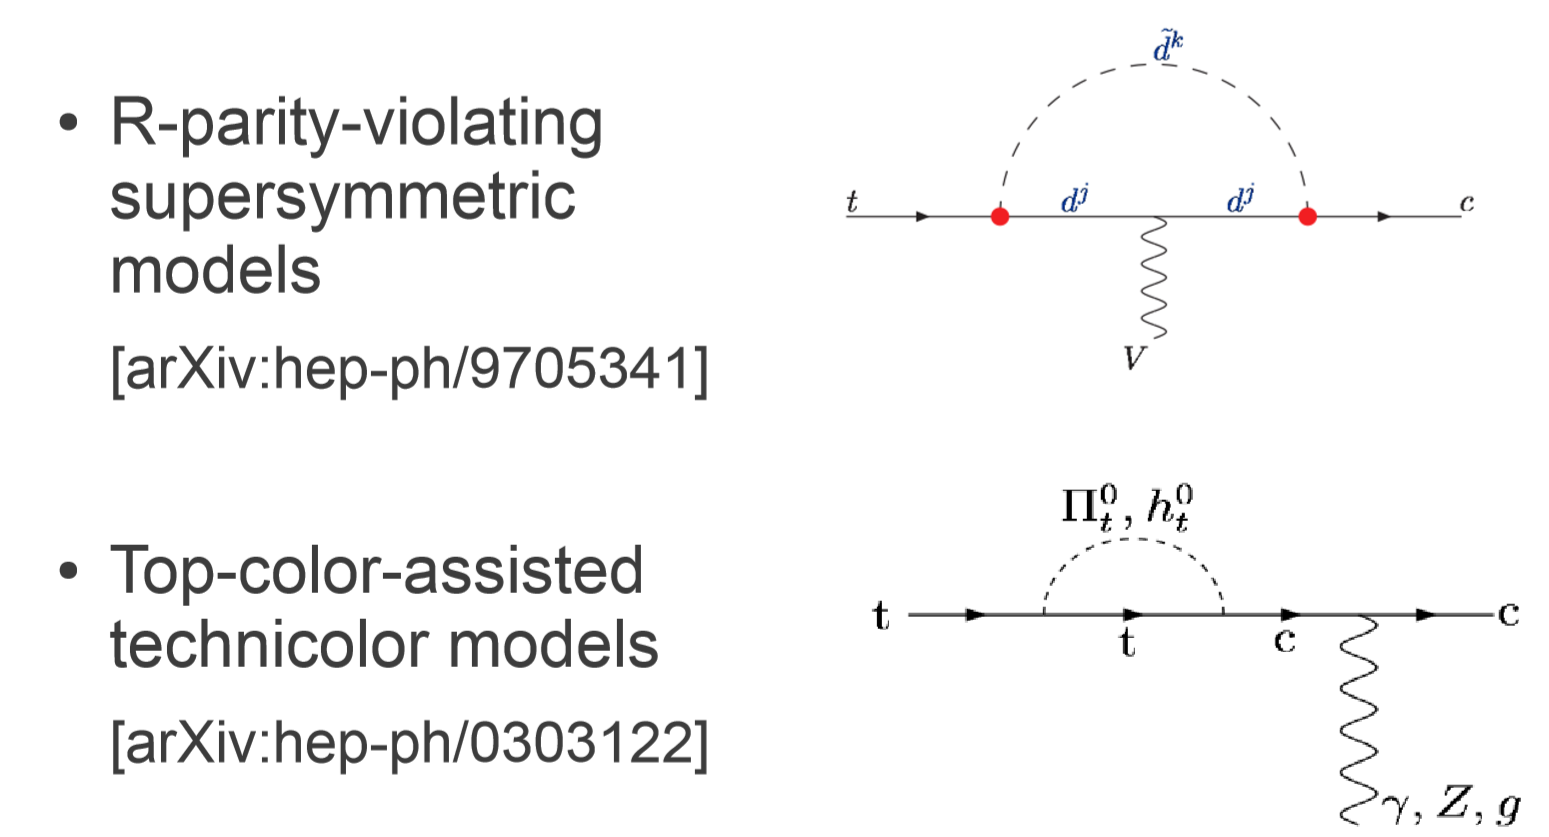
\includegraphics[width=1.\textwidth]{../../ThesisImages/BSMDiagrams.png}
}

\frame{\frametitle{Jets/AntiKT}

\[ d_{ij} = min(\frac{1}{p_{ti}^2},\frac{1}{p_{tj}^2}) \frac{\Delta_{ij}^2}{R^2}
\]
\[ d_{iB} = \frac{1}{p_{ti}^2}
\]
\[ \Delta_{ij}^2 = (\eta_i -\eta_j )^2 + (\phi_i - \phi_j )^2
\]
\begin{itemize}
\item Find minimum of entire set of $\{ d_{ij},d_{iB} \}$
\item If $d_{ij}$ is the minimum particles i,j are combined into one particle and removed from the list of particles
\item If $d_{iB}$ is the minimum i is labelled as a final jet and removed from the list of particles
\item Repeat until all particles are part of a jet with distance between jet axes $\Delta_{ij}$ is greater than R
\end{itemize}
}

\frame{\frametitle{B-tagging}
\centering
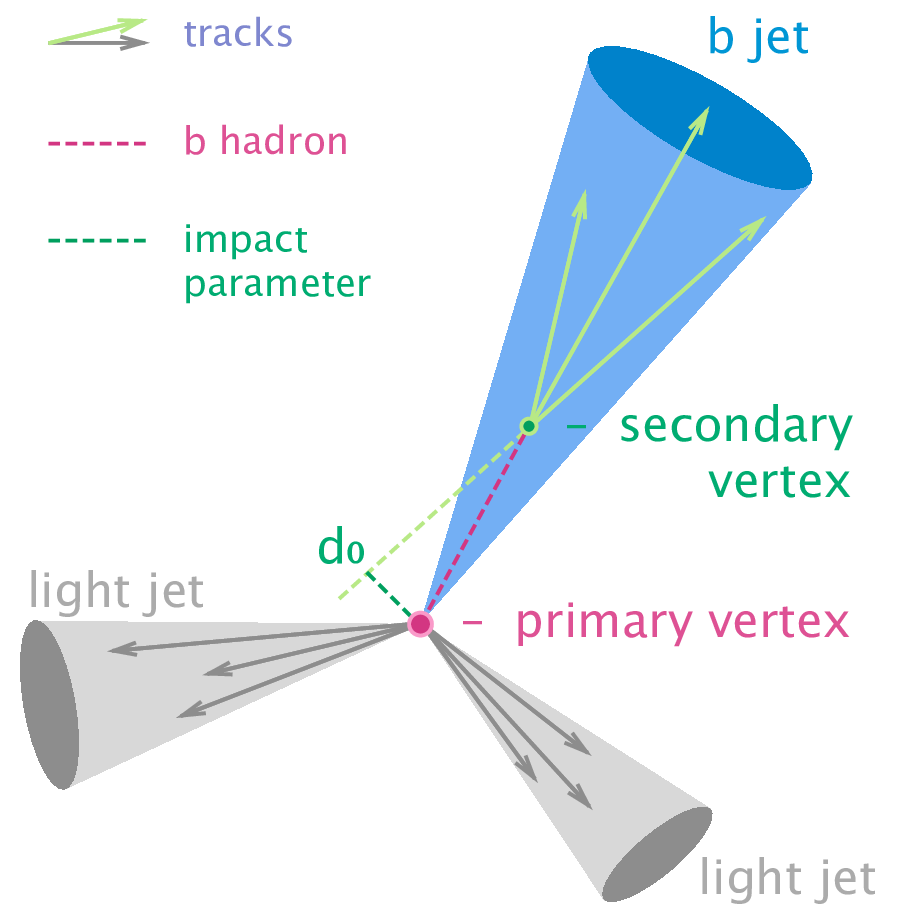
\includegraphics[height=.8\textheight]{../../ThesisImages/B-tagging_diagram.png}

}
\frame{\frametitle{}
\[ \mathcal{L}^{eff}_{tq\gamma} = - e \bar{c} \frac{i \sigma^{\mu\nu}q_{\nu}}{m_t}(\lambda^{L}_{ct}P_L + \lambda^{R}_{ct}P_{R}) t A_{\mu} +H.c.
\]
}

\end{document}

%36.070
